\chapter{Background}\label{chapter:background}

This opening chapter covers the technical background needed to read and understand this thesis. Besides a short introduction into modern cryptography schemes and advanced key exchange concepts, the emergence and consequences of quantum computers are explained. Finally, this chapter discusses isogeny-based cryptography -- the theoretical background of this thesis.
\\\\
In modern cryptography one can distinguish between \textit{symmetric} and \textit{asymmetric} encryption schemes. While in a \textit{symmetric} scheme the decryption and encryption of data is processed with the same key, \textit{asymmetric} protocols introduce a key pair for every participant: A public key for encryption and a private key for decryption. The public key of \textit{asymmetric} protocols is, as the name suggests, public to everyone. However, the private key needs to be secret and nobody but the owner has knowledge about the private key.

\subsubsection{Symmetric Cryptography}

\autoref{fig:symmetric-encryption} shows a simple symmetric encryption scheme. First, a plaintext is encrypted using a symmetric encryption algorithm and a secret key. The resulting ciphertext text is transported to the receiver, where it is decrypted using the appropriate decryption algorithm and the same secret key. The red section in the middle represents an insecure channel (e.g. the internet), where attackers may read or modify data. Since for encryption and decryption the same secret key is used, the exchange of the key through that insecure channel is critical: Somehow the symmetric key needs to be transported securely to the receiver of the ciphertext.

\begin{figure}[htpb]
	\centering
	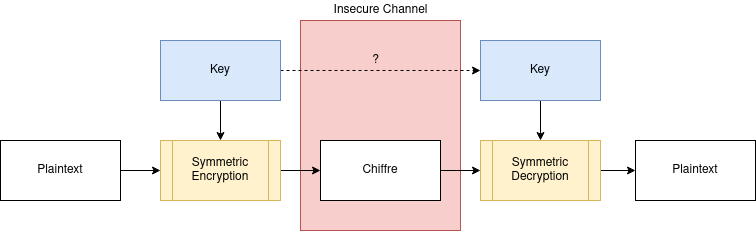
\includegraphics[width=0.8\textwidth]{background/symmetric_encryption}
	\caption[Symmetric encryption scheme]{Simple symmetric encryption scheme: Encryption and decryption algorithm use the same key.} \label{fig:symmetric-encryption}
\end{figure}

In the following, symmetric decryption and encryption is expressed in a more formal way. The common key \textit{k} is used for encryption \textit{\gls{Enc}} and decryption \textit{\gls{Dec}}, \textit{p} is the plaintext and \textit{c} is the ciphertext:

\begin{align*}
\gls{Enc}(p, k) = c\\
\gls{Dec}(c, k) = p
\end{align*}

\subsubsection{Asymmetric Cryptography}

In asymmetric cryptography each participating subject needs to generate a key pair which consist of a private key and a public key. As mentioned above, the public key needs to be public (e.g. stored in a public database or a public key server). The private key, however, is only known to the owner and is kept secret.
\autoref{fig:asymmetric-encryption} shows an example for asymmetric encryption. Assume that Alice wants to send encrypted data to Bob. Therefore, Bob created a key pair and published his public key. Alice requests Bob's public key (e.g. from a public database) and uses it to encrypt the data. Once Bob received the ciphertext, he uses his secret private key for decryption in order to retrieve the original  plaintext. In this thesis, the term \textit{public-key encryption}, \textit{PKE} and \textit{public-key algorithm} are used as a synonyms for asymmetric cryptography.

\begin{figure}[htpb]
  \centering
  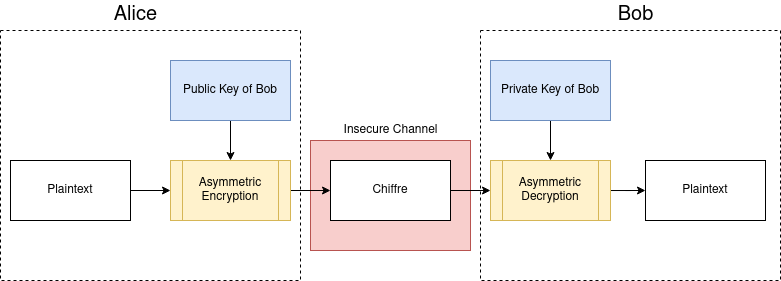
\includegraphics[width=0.8\textwidth]{background/asymmetric_encryption}
  \caption[Asymmetric encryption scheme]{Asymmetric encryption scheme: Encryption and decryption algorithm use different keys.} \label{fig:asymmetric-encryption}
\end{figure}

To formalize this procedure, again assume \textit{p} as plaintext and \textit{c} as ciphertext. The generated key pair of Bob consists of a private key for decryption ($d_{Bob}$) and a public key for encryption ($e_{Bob}$).

\begin{align*}
\gls{Enc}(p, e_{Bob}) = c\\
\gls{Dec}(c, d_{Bob}) = p
\end{align*}
\\
In contrast to \textit{symmetric} encryption, no secret key needs to be exchanged. However, the encryption and decryption of data using \textit{asymmetric} encryption require intensive mathematical computations. Hence, the encryption of big sets of data using asymmetric encryption is not efficient.\\
One the other hand, \textit{symmetric} encryption algorithms are usually based on simple operations, such as bit shifting or XOR. This can be implemented efficiently in software and hardware. Thus, the practical relevance of \textit{symmetric} encryption is enormous~\parencite{ITSicherheit}.
\\
As stated above, securely exchanged keys are a precondition for the use of efficient \textit{symmetric} encryption schemes. In order to exchange arbitrary keys securely, two major key exchange protocols are available.

\section{Key Exchange}
This section describes and compares the major protocols to establish a shared secret between two communicating subjects: The \textit{Diffie-Hellman Key-Exchange} and a \textit{Key Encapsulation Mechanism}.

\subsection{Diffie-Hellman Key-Exchange}

The Diffie-Hellman key exchange was introduced by Whitfield Diffie and Martin Hellman in 1976 ~\parencite{diffie1976new}. This protocol creates a shared secret between two subjects. The resulting shared key of the protocol is calculated decentralized and is never transported through an insecure channel.

\subsubsection{Protocol}

The classical Diffie-Hellman key exchange assumes that Alice and Bobs want to create a shared secret key. Therefore, they agree on a big prime $p$ and $g$, which is a primitive root modulo $p$\footnote{The primitive root modulo $p$ is a generator element for the set S = $\{1, 2, ... , p-1\}$~\parencite{ITSicherheit}.}. Both, $p$ and $g$ are not secret and may be known to the public~\parencite{watjen2018kryptographie}.

\begin{enumerate}
	\item Alice choses a random $a \in \{1, 2, ... , p-2\}$ as private key. 
	\item Alice calculates the public key $A = g^a\bmod p$.
	\item Bob choses a random $b \in \{1, 2, ... , p-2\}$ as private key. 
	\item Bob calculates the public key $B = g^b\bmod p$.
	\item Alice and Bob exchange their public keys $A$ and $B$.
	\item Alice calculates: 
	      \begin{equation}
	      	\begin{split}
	      		k_{AB} & = B^a\bmod p \\
	      		& = (g^b mod p)^a\bmod p \\
	      		& = g^{b a}\bmod p \\
	      		& = g^{a b}\bmod p
	      	\end{split}
	      \end{equation}
	\item Bob calculates: 
	      \begin{equation}
	      	\begin{split}
	      		k_{AB} & = A^b\bmod p \\
	      		& = (g^a\bmod p)^b\bmod p \\
	      		& = g^{a b}\bmod p
	      	\end{split}
	      \end{equation}
	\item Alice and Bob created the shared secret \gls{k_ab}. Note that only the public keys of Alice and Bob were sent through an insecure channel. The generated secret was calculated locally by Alice and Bob, respectively.
\end{enumerate}

This procedure can also be illustrated in the following diagram emphasizing the commutative properties of the protocol. It does not make any difference which function is applied first to the starting point $g$ ($x \to x^a$ or $x \to x^b$). The result is the same, since $g^{ab} = g^{ba}$.

\begin{figure}[htpb]
  \centering
  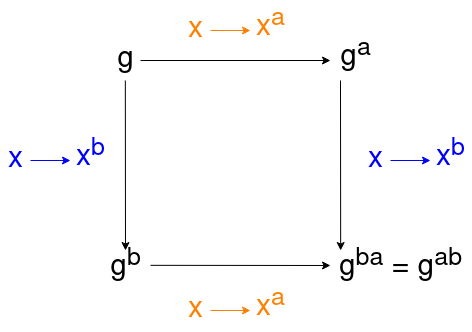
\includegraphics[width=0.5\textwidth]{background/diffie_hellman}
  \caption[Diffie-Hellman diagram]{Diffie-Hellman diagram - both paths lead to the same result.}
  \label{fig:diffie_hellman}
\end{figure}

\subsubsection{Security}
The security of the Diffie-Hellman protocol is based on the challenge: Given the public generator element $g$, the public key of Alice $g^a$ and the public key of Bob $g^b$, compute $g^{ab}$.
If an attacker wants to compute $g^{ab}$, she needs to compute the private keys $a$ and $b$ of Alice and Bob. Since only the public keys $A=g^a$ and $B=g^b$ are exchanged, it suffices to compute:
\begin{equation*}
\begin{split}
b &= \log_g B \bmod p\\ 
a &= \log_g A \bmod p
\end{split}
\end{equation*}
\\
Hence, the security of the classical Diffie-Hellman key exchange is based on the discrete logarithm problem considered difficult to be solved by classical computers (see \autoref{discrete_log_problem}). However, if an attacker is able to solve this challenge, this would neither compromise any keys from the past nor any future keys of the communication (this is called \textit{perfect forward secrecy}, short \textit{\gls{PFS}}~\parencite{ITSicherheit}). Another Diffie-Hellman handshake would challenge the attacker with the discrete logarithm problem again. Thus, the Diffie-Hellman key exchange may be used as efficient \gls{PFS} protocol when keys are renewed regularly.\\
In modern cryptography elliptic curves are often used to increase the security of the Diffie-Hellman key exchange (\gls{ECDH}). The participants have to agree on an elliptic curve and a point $P$ on that curve. In order to generate a shared secret \gls{k_ab} \gls{ECDH} follows the same principles as described above. However, the protocol is adopted to work on elliptic curves. The advantage of \gls{ECDH} is the increased security strength while using the same key size as the classical Diffie-Hellman protocol~\parencite{ITSicherheit}.
\\
Note that the introduced protocol does not authenticate the participating subjects and does not guarantee integrity. Thus, this simple protocol may be exploited by a Man-In-The-Middle attack. A more advanced protocol using certificates and signed messages can be implemented, to guarantee authentication and integrity~\parencite{ITSicherheit}.

\subsection{Key Encapsulation}

A Key Encapsulation Mechanism (\gls{KEM}) transmits a previously generated symmetric key to another subject. \glspl{KEM} usually use asymmetric key pairs in order to encrypt the generated symmetric key. In the following, the concept of \glspl{KEM} is illustrated by  \gls{rsa_kem} using \gls{RSA} key pairs to transmit a shared secret of length $n$ from Alice to Bob \parencite{rsakem}:

\begin{enumerate}
\item Bob generates a \gls{RSA} key pair (public key $e_{Bob}$ and private key $d_{Bob}$) and transmits the public key to Alice.
\item Alice generates a random secret key \gls{k_ab}:
\begin{equation*}
k_{AB} = random(n)
\end{equation*}
\item Alice maps this secret to an integer $m$, using a well-defined mapping function $h$:
\begin{equation*}
m = h(k_{AB})
\end{equation*}
\item Alice encrypts $m$ with Bobs public key using the \gls{RSA} encryption algorithm and transmits $c$ to Bob.
\begin{equation*}
c = RSA_{enc}(m, e_{Bob})
\end{equation*}
\item Bob decrypts the received ciphertext $s$ to obtain the integer $m$:
\begin{equation*}
m = RSA_{dec}(c, d_{Bob})
\end{equation*}
\item Finally, bob uses the inverse mapping function $h^{-1}$ to retrieve the shared secret:
\begin{equation*}
k_{AB} = h^{-1}(m1)
\end{equation*}

\end{enumerate}

\subsubsection{Security}
If an attacker wants to compute \gls{k_ab} it is necessary to break the \gls{RSA} encryption $RSA_{enc}(m, e_{Bob})$ in order to reveal $m$. Applying the inverse mapping function $h^{-1}$ then yields the secret key \gls{k_ab}. In order to break the \gls{RSA} encryption it is sufficient to compute the private key of Bob given his public key. This computation is assumed to be equally demanding as solving the factorization problem (see \autoref{factorization_problem}) for big numbers~\parencite{rsa2005problem}.\\
Note that once an attacker was able to compromise Bobs private key, all following exchanged shared secrets \gls{k_ab} are compromised as well. Thus, this protocol does not ensure perfect forward secrecy (\gls{PFS}).

\subsection{Differences}
Both presented protocols securely share a symmetric encryption key between two communicating subjects. However, there are some differences between \gls{KEM} and Diffie-Hellman. Firstly, while \glspl{KEM} transmit a shared secret from one subject to another, the calculation in the Diffie-Hellman protocol is decentralized. Thus, the shared secret will never be send through an insecure channel.\\
Secondly, \gls{KEM} relies on a long-term asymmetric key pair which is used to encapsulate and decapsulate the randomly chosen shared secret. If the private key is compromised by an attacker, all following symmetric encrypted communication could be revealed. On the contrary, a compromised Diffie-Hellman key exchange would only affect the messages which are encrypted using the secret resulting from that single Diffie-Hellman handshake. All following \gls{DH} key exchanges are not compromised from the previously compromised exchange. Thus, \gls{DH} key exchanges might be used as the basis of a \gls{PFS} protocol.\\
Thirdly, KEMs can be used offline: Since one subject (e.g the sending subject) chooses the secret key, data calculation and encryption can be performed without any previous communication with the receiver. Thus, no synchronization between the subjects is necessary to exchange encrypted data.
\newpage
\section{Post-Quantum Cryptography}
This section introduces the term \textit{quantum computer} and describes its consequences on modern cryptography. In the following, a \textit{classical computer} refers to a non-quantum computer which can be simulated by a Turing machine. In contrast to \textit{classical computer} the term \textit{quantum computer} describes a machine using quantum mechanical phenomena to perform computations. It is important to note that quantum computers can simulate classical computers~\parencite{nielsen2002quantum}. In addition, classical computer are able to simulate quantum computers with exponential time overhead~\parencite{nielsen2002quantum}. Thus, classical and quantum computers can calculate the same class of functions. However, quantum computers enable operations allowing much faster computation in some cases~\parencite{nielsen2002quantum}.\\
In the past, scientists queried whether large-scale quantum computer are physically possible. It was argued that the underlying quantum states are too fragile and hard to control~\parencite{chen2016report}. Today, quantum error correction codes are known, putting large-scale quantum computers within the realms of possibility~\parencite{lidar2013quantum}. However, it is still a major engineering challenge from a laboratory approach to a general-purpose quantum computer that involves thousands or millions of logical qubits~\parencite{chen2016report}.
\\\\
The security of modern asymmetric cryptographic primitives is usually based on difficult number theoretic problems, e.g. the discrete logarithm problem (\gls{DH}, \gls{ECDH}) or the factorization problem (\gls{RSA})~\parencite{chen2016report}. While these problems are theoretically solvable, the computation on classical computers claim an impractical amount of resources. In 2019, scientists solved the factorization problem for a 240 digit integer in about 900 core-years on a classical computer (one core year corresponds to running a CPU for a full year)~\parencite{boudot2795}. In the following, the discrete logarithm problem and the factorization problem are described.

\subsubsection{Discrete Logarithm Problem} \label{discrete_log_problem}
The discrete logarithm problem consists in the following challenge \parencite{beutelspacher2010diskrete}: Given a prim $p$ and two integers $g$ and $y$. Find an integer $x$, such that
\begin{equation*}
\begin{split}
&y = g^x \bmod p \\
\iff &x = \log_g y \bmod p
\end{split}
\end{equation*}
Up to this date, it remains still unknown if a classical computer is able to compute the general discrete logarithm problem in polynomial time. Thus, the discrete logarithm problem is considered difficult to be solved by classical computers~\parencite{beutelspacher2010diskrete}. This assumption makes the discrete logarithm problem an attractive basis for various cryptographic primitives: \gls{DSA}, ElGamal, classical Diffie-Hellman, and Elliptic Curve Diffie-Hellman employ the hardness of the discrete logarithm problem in order to secure their algorithms.

\subsubsection{Factorization Problem} \label{factorization_problem}

Given two large primes p and q, it is easy to compute their respective product:
\begin{equation*}
n = p \cdot q
\end{equation*}
For a given $n$, however, it is difficult to find the prime factors $p$ and $q$. The computation of the prime factorization for a given integer $n$ is called the factorization problem~\parencite{ITSicherheit}. For large numbers $n$ no efficient algorithm for classical computers is known to solve this challenge~\parencite{ITSicherheit}. The most famous cryptographic protocol which builds upon the hardness of the factorization problem is \gls{RSA}.

\subsection{Impact of Quantum Computers on Cryptography}

As stated above, quantum computers enable new operations which accelerate certain algorithms. Two quantum algorithms which have enormous consequences on modern cryptography are \textit{Shor's algorithm}~\parencite{shor1994algorithms} and \textit{Grover's algorithm}~\parencite{grover1996fast}.

\subsubsection{Shor's Algorithm}
Peter Shor published \textit{"Algorithms for quantum computation: discrete logarithms and factoring"} in 1994~\parencite{shor1994algorithms}. In this publication he demonstrated that the factorization problem and the discrete logarithm problem can be solved in polynomial time on quantum computers. Both problems form the basis of many public-key systems (\gls{RSA}, \gls{DH}, \gls{ECDH}, ...) used intensively in modern communication systems. Hence, a quantum computer running \textit{Shor's algorithm} would qualify for the assumption of most asymmetric encryption schemes and thus break their security.


\subsubsection{Grover's Algorithm}
The second algorithm impacting computer security was published by Lov Grover in 1996 (\textit{"A fast quantum mechanical algorithm for database search"}, \parencite{grover1996fast}) - also referred to as \textit{Grover's algorithm}. The algorithms solves the problem of finding an element $y$ in a set $S$ (e.g. a database) where $|S| = N$. On a classical computer an algorithm solving this problem runs in $\mathcal{O}(N)$. However, \textit{Grover's algorithm} has complexity $\mathcal{O}(\sqrt{N})$~\parencite{nielsen2002quantum}.\\
In contrast to public-key systems that rely on hard mathematical problems, symmetric encryption schemes rely in particular on the secrecy of a randomly generated key. 
Thus, to break symmetric encryption, one can perform a brute-force attack on the symmetric key. \textit{Grover's algorithm} offers a square root speed-up on classical brute-force attacks~\parencite{mavroeidis2018impact}. Assume a randomly generated $n$-bit key. A classical brute force algorithm takes $\mathcal{O}(2^n)$ steps, which is considered to be safe for a big $n$ (e.g. $n=128$). \textit{Grover's algorithm} speeds up this attack to $\mathcal{O}(\sqrt{2^n})$ = $\mathcal{O}(2^{n/2})$ steps~\parencite{mavroeidis2018impact}. For $n=128$ this results in a security level of 64-bit ($2^{128/2}=2^{64}$)~\parencite{mavroeidis2018impact}. Note that \gls{NIST} considers a security-level of at least 112-bits as secure ~\parencite{barker2019transitioning}.  However, the complexity is still exponential and with a growing key size $n$ the security can be increased further (e.g. doubling key size $n$ is sufficient to restore previous security). Thus, \textit{Grover's algorithm} forces symmetric encryption schemes to increase their key size in order to stay secure.
\\\\
Summing up, quantum computers make use of quantum mechanical phenomena in order to solve mathematical problems which are assumed to be difficult for classical computers. As a result large-scale quantum computers might break many algorithms of modern \textit{asymmetric} cryptography and enforce increased key sizes for \textit{symmetric} encryption schemes. The following table form the \gls{NIST} \textit{"Report on Post-Quantum Cryptography"} \parencite{chen2016report} demonstrates the impact of quantum computers on modern encryption schemes:

\begin{table}[H]
  \centering
  \begin{tabular}{|K{3cm}|K{3cm}|K{4cm}|K{4cm}|}
	\hline
    \rowcolor{lightgray!50}
      \textbf{Cryptographic} \textbf{algorithm} & \textbf{Type} & \textbf{Purpose} & \textbf{Impact from} \textbf{ quantum computer} \\
	\hline
      \gls{AES} & Symmetric key & Encryption & Larger key sizes needed \\
    \hline
      \gls{SHA} & --- & Hash functions & Larger output needed \\
    \hline
      \gls{RSA} & Public key & Signatures, key establishment & No longer secure \\
	\hline      
      \gls{DSA} & Public key & Signatures, key exchange & No longer secure \\
    \hline
      \gls{ECDH}, \gls{ECDSA} & Public key & Signatures, key exchange & No longer secure \\
    \hline
  \end{tabular}
  \caption[Impact of quantum computers on modern encryption schemes]{Impact of quantum computers on modern encryption schemes (adopted from \parencite{chen2016report}).}\label{tab:impact}
\end{table}

In contrast to this development in modern cryptography \gls{NIST} states~\parencite{chen2016report}:
\begin{quote}
\textit{"In the last three decades, public key cryptography has become an indispensable component of our global communication digital infrastructure. These networks support a plethora of applications that are important to our economy, our security, and our way of life, such as mobile phones, internet commerce, social networks, and cloud computing. In such a connected world, the ability of individuals, businesses and governments to communicate securely is of the utmost importance."}
\end{quote}
This statement emphasizes the urgency and need of new asymmetric encryption schemes. As a consequence, \gls{NIST} initiated a process to standardize quantum-secure public-key algorithms~\parencite{nist2017callforproposals}. This is called \textit{post-quantum cryptography}, since the objectives of the submitted procedures is to stay secure against a large-scale quantum computer. In July 2020, Round 3 of this standardization process was announced. Different approaches for quantum-resistant algorithms have been proposed. This thesis focus on isogeny-based cryptography (section \ref{sec:isogeny-based_crypto}). Other classes of post-quantum cryptography are described for completeness in the following section \ref{sec:classes_pqc}.

\subsection{Classes of Post-Quantum Cryptography} \label{sec:classes_pqc}

This section provides an overview over important post-quantum cryptography classes: Lattice-based, multivariate and code-based cryptography as well as hash-based signatures are briefly presented. 
\subsubsection{Lattice-based Cryptography}
Lattice-based cryptography is -- as the name suggests -- based on the mathematical construct of lattices\footnote{A lattice $l$ is a subgroup of $\mathbb{R}^n$. In the context of cryptography usually integer lattices are considered: $l \subseteq \mathbb{Z}^n$ \parencite{chi2015lattice}.}. There are different computational optimization problems involving lattices that are considered difficult to be solved even by quantum computers~\parencite{chi2015lattice}. In 1998, \gls{NTRU} was published as the first public-key system based on lattices ~\parencite{hoffstein1998ntru}. Since then \gls{NTRU} was continuously improved resulting in NTRUencrypt (public-key system) and \gls{NTRUsign} (digital signing algorithm). Furthermore, a fully homomorphic encryption scheme based on lattices was published in 2009~\parencite{gentry2009fully}.\\
Lattice-based cryptography is characterized by simplicity and efficiency \parencite{chen2016report}. However, lattices encryption schemes have problems to prove security against known cryptoanalysis \parencite{chen2016report}.
\subsubsection{Multivariate Cryptography}
Multivariate cryptography are public key systems that are based on multivariate polynomials (e.g. $p(x,y)=x+2y$) over a finite field $\mathbb{F}$. The proof that solving systems of multivariate polynomials are NP-hard~\parencite{hartmanis1982computers} is the basis of their security. This makes multivariate public key systems attractive for post-quantum cryptography; especially their short signatures make them a candidate for quantum-secure digital signature algorithms~\parencite{ding2017current}, e.g. the Rainbow signature scheme~\parencite{ding2005rainbow}.
\subsubsection{Code-based Cryptography}
Code-based cryptographic primitives are build upon error-correcting codes. A public key system using error-correcting codes uses a public key to add errors to a given plaintext resulting in a ciphertext. Only the owner of the private key is able to correct these errors and to reconstruct the plaintext~\parencite{bernstein2017post}. \gls{McEliece}, published in 1978, was the first of those systems and it has not been broken until today~\parencite{mceliece1978public}. On the other hand, code-based cryptography requires large key sizes~\parencite{bernstein2017post}.\\
Besides asymmetric cryptography, code-based schemes have been proposed for digital signatures, random number generators and cryptographic hash functions~\parencite{bernstein2017post}.
\subsubsection{Hash-based Signatures}
Hash-based signatures refer to the construction of digital signatures schemes based on hash functions. Thus, the security of theses primitives is based on the security of the underlying hash function and not on hard algorithmic problems~\parencite{bernstein2017post}. Since hash functions are widely deployed in modern computer systems, the security of hash-based signatures is well understood~\parencite{chen2016report}.\\
The initially developed One-Time Signatures have the downside that a new public key pair is needed for each signature~\parencite{becker2008merkle}. In 1979, Merkle introduced the Merkle Signature Scheme (\gls{MSS}) which uses one public key for multiple signatures~\parencite{merkle1979secrecy}. Further improvements of \gls{MSS} introduced public keys usable for $2^{80}$ signatures. However, this also leads to longer signature sizes~\parencite{becker2008merkle}.

\section{Isogeny-based Cryptography} \label{sec:isogeny-based_crypto}
Isogeny-based cryptography was proposed in 2011 as a new cryptographic system that might resists quantum computing~\parencite{jao2011towards}. Besides describing isogeny-based cryptography, the authors also provided a reference implementation for a \gls{PKE} and a \gls{KEM} based on isogenies. This implementation is called \textit{\gls{SIKE}}~\parencite{sike2020spec}. Isogeny-based cryptography benefits from small key sizes compared to other post-quantum cryptography classes, however, their performance is comparatively slow~\parencite{sike2020spec}. The security of these primitives is based on finding isogenies between supersingular elliptic curves.\\
In the following, the problem is firstly roughly illustrated. It is not indented to provide exact mathematical details about isogeny-based cryptography, since that would be beyond the scope of this thesis. However, one might become an intuition for supersingular isogenies. Subsequently, the central component of isogeny-based cryptography - namely the Supersingular Isogeny Diffie-Hellman (\gls{SIDH}) - is described. Finally, details of the reference implementation \gls{SIKE} are given and the security of \gls{SIDH} is considered.

\subsection{Mathematics}
This section is adopted from~\citetitle{urbanik2017friendly}~\parencite{urbanik2017friendly} and~\citetitle{costello2019supersingular}~\parencite{costello2019supersingular}.\\
Isogeny-based cryptography works on supersingular elliptic curves. To be more precise: It is based on isogenies between supersingular elliptic curves.
\\
In the context of elliptic curves one can calculate a quotient of an elliptic curve $E$ by a subgroup $S$. Essentially, this means to construct a new elliptic curve $E$\textbackslash $S$.
Besides this new curve, the procedure also yields a function $\phi_S: E \to E \backslash S$ which is called an \textit{isogeny}. Carefully chosen elliptic curves E have a wide range of subgroups which can be used to construct many isogenies.
\\
Supersingular elliptic curves are a special type of elliptic curves having properties that are useful for cryptography. Since supersingular elliptic curves can be seen as subset from ordinary elliptic curves, they can also be used to calculate isogenies between them, as described above.
\\
The idea behind isogeny-based cryptography might be illustrated as follows:

\begin{enumerate}
\item Start with a known curve $E$ and build an isogeny to an arbitrary reachable curve $E_A$.
\item This yields the isogeny $\phi_A: E \to E_A$ which is used as private key.
\item The curve $E_A$ is used as part of the public key.
\end{enumerate}
Usually, in asymmetric asymmetric cryptography the hard mathematical problem consists in computing the private key while knowing the public key. To be more precise: Find the isogeny $\phi_A: E \to E_A$ while knowing curves $E$ and $E_A$ is considered to be a quantum-resistant challenge. In literature, this is formally defined as \textit{\gls{SIDH} problem}~\parencite{sike2020spec}. 
\\
This key pair, however, is not used to decrypt or encrypt data. In fact, the procedure is very similar to the previously introduced Diffie-Hellman key exchange where the key pair is used to establish a shared secret between two communication partners.
In its core, isogeny-based cryptography creates a shared secret via a Diffie-Hellman like procedure. This is called \textit{Supersingular Isogeny Diffie Hellman (\gls{SIDH})}.

\subsection{Supersingular Isogeny Diffie-Hellman (\gls{SIDH})}

In the previous section the underlying mathematical idea of isogeny-based cryptography was illustrated. The described key generation can be extended to a key exchange primitive which has strong similarity to the classical Diffie-Hellman key exchange. The SIDH key exchange is represented by the following protocol.\\
Starting point of \gls{SIDH} is a publicly known supersingular elliptic curve E. 

\begin{enumerate}
\item Alice creates an isogeny $\phi_A$ (private key) which leads to curve $E_A$ (part of Alice's public key).
\item Bob creates an isogeny $\phi_B$ (private key) which leads to curve $E_B$ (part of Bob's public key).
\item Alice and Bob exchange their public keys.
\item Bob computes $\phi_B'$ (using additional information from the public key of Alice) and applies $\phi_B'$ to the received $E_A$. This results in $E_{AB}$
\item Alice computes $\phi_A'$ (using additional information from the public key of Bob) and applies $\phi_A'$ to the received $E_B$. This results in $E_{AB}$
\item Alice and Bob share the  common secret $E_{AB}$.
\end{enumerate}


 \autoref{fig:diffie_hellman} above showed the commutative property of the classical Diffie-Hellman protocol. The same diagram can be drawn for the Diffie-Hellman based on supersingular isogenies (see \autoref{fig:sidh}):
\begin{figure}[H]
  \centering
  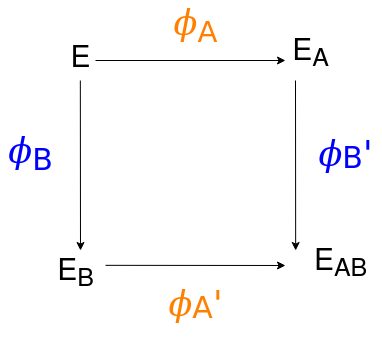
\includegraphics[width=0.5\textwidth]{background/sidh}
  \caption[Supersingular Isogeny Diffie-Hellman diagram]{Supersingular Isogeny Diffie-Hellman procedure - both paths lead to the same result $E_{AB}$. Note the different isogenies $\phi_{A}'$ and $\phi_{B}'$ that are applied in each second step of the diagram. The reason for this lies in the mathematics of supersingular isogenies. In order to construct $\phi_{X}'$ or $\phi_{B}'$ the public key of each communication partner provides additional information besides the curve $E_A$ or $E_B$.~\parencite{costello2016gentle}}
  \label{fig:sidh}
\end{figure}

\subsection{Implementation Details}\label{sec:sidh_implementation}

The implementation details described in this subsection are based on \textit{\gls{SIKE}}~\parencite{sike2020spec}, the first proposed supersingular isogeny-based cryptography. The following explanations also illustrate the connection between SIDH and isogeny-based \gls{PKE} and \gls{KEM}.\\
The reference implementation of \gls{SIKE} provides two fundamental functions: \textit{isogen} and \textit{isoex}. Both are used, to implement the previously introduced \gls{SIDH} algorithm. Note that the secret key \textit{sk} is represented as a random integer. Moreover, the used parameters that represent the applied supersingular curve are also passed to \textit{isogen} and \textit{isoex}. For simplicity, this is not listed here, however the exact parameter sets for all curves are listed in the specification of \gls{SIKE}~\parencite{sike2020spec}.

\begin{table}[H]
  \centering
  \begin{tabular}{|K{3cm}|K{4cm}|K{4cm}|}
	\hline
    \rowcolor{lightgray!50}
      \textbf{Function} & \textbf{Input} & \textbf{Output} \\
	\hline
      \textit{isogen} & \parbox[t]{4cm}{\centering parameter set \textit{param}\\party \textit{p}\\ secret key \textit{sk}} & \makecell{public key pk} \\
     \hline
      \textit{isoex} & \parbox[t]{4cm}{\centering parameter set \textit{param}\\party \textit{p}\\ secret key \textit{sk}\\ public key \textit{pk}} & shared secret \textit{sec}\\
     \hline
  \end{tabular}
   \caption[Core functions of the \gls{SIKE} reference implementation]{Core functions of the \gls{SIKE} reference implementation.}\label{tab:sike_core_functions}
\end{table}
The function \textit{isogen} takes a secret key (random integer), the parameter set and the party (Alice or Bob) as input and generates the public key. The shared secret is generated by \textit{isoex} taking the own secret key and the foreign public key as input. Additionally \textit{isoex} also expect the used parameter set and the party of the key exchange. The party needs to be specified since Alice and Bob do not use the same logic to generate their keys and the shared secret. The reason for this lies in the mathematical foundation of isogeny based cryptography. The \gls{SIDH} key exchange procedure with respect to \textit{isogen} and \textit{isoex} works as follows:
\begin{figure}[H]
  \centering
  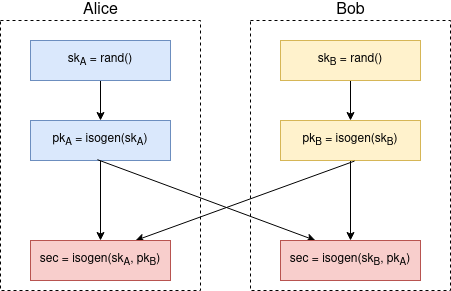
\includegraphics[width=0.6\textwidth]{background/sike_sidh}
  \caption[\gls{SIDH} based on \textit{isogen} and \textit{isoex}]{\gls{SIDH} based on \textit{isogen} and \textit{isoex}: After generating a random secret key \textit{sk} each subject computes its public key \textit{pk}. After the exchange of public keys each subject finally calculates the shared secret \textit{sec}. It is important that both parties use the same parameter set \textit{param}} \label{fig:sike-sidh}
\end{figure}
Besides this key exchange algorithm, \gls{SIKE} provides a complete asymmetric encryption scheme  and a key encapsulation mechanism  ~\parencite{sike2020spec}. Both of these schemes build upon the here described \gls{SIKE} core functions \textit{isogen} and \textit{isoex}.

\subsubsection{Isogeny-based \gls{PKE}}
The isogeny-based public-key encryption system (\gls{PKE}, \autoref{fig:sike-pke}) consists of three algorithms. The authors of \gls{SIKE} state, that their \gls{PKE} scheme is a modification of the classical hashed ElGamal scheme by replacing classical Diffie-Hellman procedure with quantum-secure \gls{SIDH} \parencite{sike2020spec}.
\begin{enumerate}
\item \textit{Gen} generates a key pair ($sk_A$,$pk_A$). Firstly, the private key is chosen at random. The public key is then derived from the random private key using \textit{isogen}.
\item \textit{\gls{Enc}} encrypts a given plaintext $m$ using a foreign public key $pk_B$ and a random $r$. Internally, the random $r$ is treated as private key: $c_0$ is derived from $r$ via \textit{isogen}. A secret is then generated by \textit{isoex} using the foreign public key $pk_B$ and the private key $r$. The hash of this secret $F(sec)$ is finally XORed with the given plaintext $m$ and saved in $c_1$. The function returns $c_0$ and $c_1$.
\item \textit{\gls{Dec}} decodes a given ciphertext ($c_0$,$c_1$) using the secret key $sk_B$. Firstly, a secret is derived by \textit{isoex} using the private key $sk_B$ and foreign public key $c_0$. The hash of this secret $F(sec)$ is XORed with the ciphertext $c_1$ returning the plaintext $m$. The function returns $m$.
\end{enumerate}
Note that the function $F$ used in \textit{\gls{Enc}} and \textit{\gls{Dec}} is a key derivation function.

\begin{figure}[H]
  \centering
  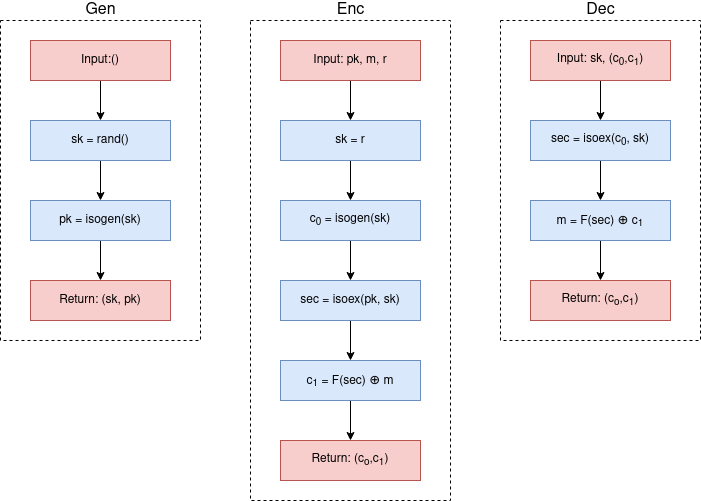
\includegraphics[width=1\textwidth]{background/sike_asym}
  \caption[Isogeny-based \gls{PKE}]
  {Isogeny-based public-key encryption (\gls{PKE}) scheme.} \label{fig:sike-pke}
\end{figure}

\subsubsection{Isogeny-based \gls{KEM}}
The construction of the isogeny-based key encapsulation mechanism (\gls{KEM}, \autoref{fig:sike-kem}) consists of three algorithms. The authors of \gls{SIKE} state to build a \textit{IND-CCA} \gls{KEM} from their \gls{PKE} \parencite{sike2020spec} (by applying a slight modification of the transformation published by Hofheinz, Hüvelsmann and Klitz \parencite{cryptoeprint:2017:604}). This essentially means, that an attacker can not distinguish two ciphertexts created by the \gls{KEM} encryption function \textit{Encaps}. The following algorithms describe how the isogeny-based \gls{KEM} is created from the isogeny-based \gls{PKE} described above. The goal of this construction is to build an \textit{IND-CCA} \gls{KEM} (see \parencite{cryptoeprint:2017:604} for details).
\begin{enumerate}
\item \textit{KeyGen} generates a key pair ($sk_A$,$pk_A$) and a secret \textit{s}. The private key $sk$ and the secret $s$ are chosen at random. The public key is derived from the random private key using \textit{isogen}.
\item \textit{Encaps} takes a given public key $pk_B$ as input and calculates a secret to share named \textit{K}. Moreover, the function returns a ciphertext \textit{c} that will be forwarded to the owner of the public key.
\item \textit{Decaps} takes a ciphertext \textit{c} and the output of \textit{Gen} as input in order to retrieve the shared secret \textit{K}.
\end{enumerate}
\begin{figure}[H]
  \centering
  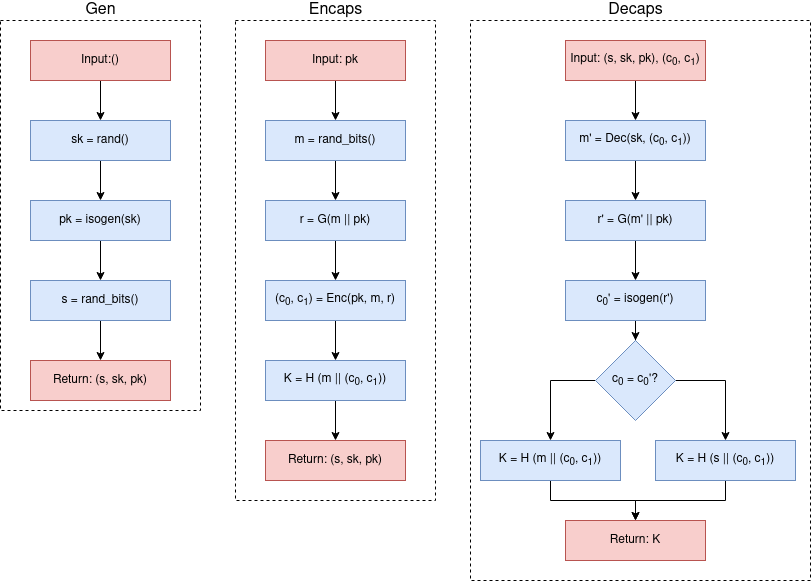
\includegraphics[width=1\textwidth]{background/sike_kem}
  \caption[Isogeny-based \gls{KEM}]
  {Isogeny-based key encapsulation mechanism (\gls{KEM}).} \label{fig:sike-kem}
\end{figure}
\subsection{Security}\label{sidh_security}
The security of isogeny-based cryptography is based on the hardness of the \textit{\gls{SIDH} problem}: Given two supersingular elliptic curves $E$ and $E'$, find an isogeny between them~\parencite{sike2020spec}. 
\\
The \gls{SIKE} reference implementation proposes different parameter sets, each supposing to ensure a \gls{NIST} defined security level. These \gls{NIST} defined security levels are:\\
\renewcommand\arraystretch{2}
\begin{tabular}{ | L{2cm} | L{13cm} | }  
\hline
    \textbf{Level 1}
    &
    Any attack breaking this security level must require resources comparable to perform a key search on a 128-bit key (e.g. AES128). \\
\hline
    \textbf{Level 2}
    &
    Any attack breaking this security level must require resources comparable to perform a collision search on a 256-bit hash function (e.g. SHA256). \\
\hline
    \textbf{Level 3}
    &
    Any attack breaking this security level must require resources comparable to perform a key search on a 192-bit key (e.g. AES192). \\
\hline
    \textbf{Level 4}
    &
    Any attack breaking this security level must require resources comparable to perform a collision search search on a 384-bit hash function (e.g. SHA384). \\
\hline
    \textbf{Level 5}
    &
    Any attack breaking this security level must require resources comparable to perform a key search on a 256-bit key (e.g. AES256). \\
\hline
\end{tabular}
\renewcommand\arraystretch{1}
\newline
The proposed parameter sets of \gls{SIKE} are named after the bit length of the underlying primes $p$. This prime $p$ is part of the parameter set itself. See \parencite{sike2020spec} for the detailed definition of each parameter set. Note that the authors of SIKE did not propose a parameter set supposed to satisfy \gls{NIST} security level 4 (SHA384).

\begin{itemize}
\itemsep0em 
	\item \texttt{p434} supposed to satisfy \gls{NIST} security level 1 (AES128)
	\item \texttt{p503} supposed to satisfy \gls{NIST} security level 2 (SHA256)
	\item \texttt{p610} supposed to satisfy \gls{NIST} security level 3 (AES192)
	\item \texttt{p751} supposed to satisfy \gls{NIST} security level 5 (AES256)
\end{itemize}
All isogeny-based cryptographic primitives presented in this chapter can be initialized with one of these parameter sets to match a certain security level. In the context of this thesis the used parameter sets are also called \textit{curves}.
\\\\
Current research suggest that the \gls{SIKE} parameter sets satisfy the defined security levels even under the assumption of currently known algorithms~\parencite{jaques2019quantum}. Therefore, the authors consider three algorithms to solve the \textit{\gls{SIDH} problem}: \textit{Tani's quantum claw finding algorithm}~\parencite{tani2009claw}, \textit{Grover's algorithm}~\parencite{grover1996fast} and a \textit{parallel collision-finding algorithm}~\parencite{van1999parallel}.
\\
Ephemeral \gls{SIDH} keys are predestined to implement quantum-secure perfect forward secret protocols ~\parencite{koziel2018high}. \gls{PFS} ensures that a compromised long-term key does not reveal past or future keys of the protocol.
\\
Side-channel attacks against isogeny-based cryptography might 1) reveal parts of the secret private key or 2) reveal parts of the public key computation. To protect against power-analysis side-channel attacks it is recommend to implement constant-time cryptography~\parencite{sike2020spec}. The authors state, however, that an attacker has \textit{"access to a wide range of power, timing, fault and various other side-channels"}. Thus, preventing isogeny-based cryptography from all side-channel attacks seems to be a challenge and is an active research area.
